\section{Reikningar}\label{ch::reikningar}

Við reikninga var miðað við eina plötu, þ.e. þegar aðskilnaður flata hefur átt sér stað. 

Byrjað var á ytri greiningu samsetningarinnar. Því ytra álag á hana er samhverft um miðju fæst að báður undir stöðukraftarnir eru $R_{A} = R_{B} = F/2$, sbr. mynd \ref{fig::forsendur}. Við útreikninga var miðað við að mesta spennur sem boltinn eða efnið þyldi væri flotmörk, þ.e. $n_y$ = 1. Mesta beygjuspenna sem hver plata þolir án þess að fara í flot er því í miðju samsetningarinnar. Út frá því má vinna mestan kraft sem hver plata þolir án þess að fara í flot.

\begin{equation}
	\sigma = \frac{M c}{I} = \frac{F l h}{4I} \Rightarrow F = \frac{4 \sigma I}{l h}
	\label{eq::1}
\end{equation}

Í jöfnu \ref{eq::1} er allt fastar nema flatartregðuvægið, I. Með því að lækka flatartregðuvægið mun mesti kraftur sem platan þolir fyrir flot minnka og því er ákveðið að bora ekki í miðja plötuna. Þessi kraftur, $F_{y,p}$, er því notaður sem lágmark þegar stærð, staðsetning og fjöldi bolta er valin. Því notum við það sem forsendur fyrir hönnun okkar að ef samsetningin í flot við minni kraft heldur en $F_{y,p}$ á einhverjum stað þá virkar sú hönnun ekki. Flatartregðuvægið fyrir ferhyrnt þversnið $I = {1 \over 12}bh^3$, því fæst sá kraftur sem lætur samsetninguna fara í flot í miðju er

\[
	F_{y,p} = \frac{4  \sigma_y I}{l h} = {\sigma_y b h^2 \over 3 l} = {210 MPa \cdot 5 mm \cdot \left(50mm\right)^2 \over 3 \cdot 200mm} = 4375N
\]

\subsection{Mismunandi tilvik semsetninga}

Þau tilvik sem þarf að skoða til viðbótar við þar sem samsetningin gefi sig eru þrenn

\begin{enumerate}
	\item Beygjuspenna á yfirborði þar sem borað verður
	\item Skerspenna sem boltar verða fyrir
	\item Leguspenna sem verkar á efnið í götunum
\end{enumerate}

Til að minnka beygjuspennu á yfirborði er ákveðið að hafa götin sem næst lóðréttum brúnum samsetningarinnar. Með því er vægisarmurinn frá undirstöðunum styttur, sem minnkar beygjuspennuna sbr. jöfnu \ref{eq::1}. Við þetta hækkar skerspennan í boltum og leguspennan í götum efnisins. Til að koma til móts við þessa spennuhækkun er ákveðið að hafa götin sem fjærst lágréttum brúnum samsetningarinnar, við það munu þær spennur lækkar, sbr. jöfnu \ref{eq::2}\cite{shigleys}.

\begin{equation}
	F_n^{''} = {M r_n \over \displaystyle\sum_{i=1}^{k} r_i^2}
	\label{eq::2}
\end{equation}

Þar sem $F_n^{''}$ er skerkraftur sem verkar á bolta n sem er í fjarlægð $r_n$ frá flatarmiðju boltanna og k er fjöldi bolta í samsetningunni. Með þessu er hægt að finna leguspennu sem virkar á efnið og skerspennu sem virka á boltana. Reiknað voru þrjú tilvik af mismunandi samsetningu. Reiknað var í hverju tilfelli kraftinn sem olli því að fyrrnefndar spennur færu í flot.

\subsubsection{Fyrsta tilvik}

Í upphafi var einföld hönnun valin, sjá mynd \ref{fig::2x6}. Vegna samhverfum um miðju er nóg að reikna aðeins fyrir annan boltann.

\begin{itemize}
	\item Beygjaspenna á yfirborði við göt
	
Jafna \ref{eq::1} er notuð við þetta en nú er flatartregðuvægið minna vegna holunar. Flatartregðuvægið er því $I = {1 \over 12}bh^3 - {1 \over 12}bd^3$. Því er sá kraftur sem veldur floti
\[
F = \frac{4 \sigma I}{l h} = {4 \cdot 210 MPa \cdot  \left({1 \over 12} \cdot 5 mm \cdot \left(50mm\right)^3 - {1 \over 12} 5 mm \cdot \left(6mm\right)^3\right) \over (160 mm + 12 mm) \cdot 50 mm} = \underline{5080N}
\] 

	\item Skerspenna í bolta

Jafna \ref{eq::2} er notuð til að finna skerkraftinn sem virkar á boltann

\[
F_1^{''} = F_2^{''} = {Mr_n \over 2r_n^2} = {{F \over 2}l \over 2 r_n} 
\]

Sá kraftur sem veldur því að skerspennan í boltanum fari uppí flotspennu

\[
\sigma = {F_1^{''} \over A_b} \Rightarrow F = {4 S_{sy} A_b r_n \over l} = {4 \cdot {660MPa \over \sqrt{3}} \cdot {\pi \left(6mm\right)^2 \over 4} \cdot 28 mm \over 200 mm} = \underline{6030N}
\]

	\item Leguspenna í efni
	
	Sá kraftur sem virkar á leguna er skerkrafturinn sem verkar á boltar, því verður leguspennan
	
\[
\sigma = {F_1^{''} \over bd} \Rightarrow F = {4 \sigma_{y} b d r_n \over l} = {4 \cdot 210 MPa \cdot 5 mm \cdot 6 mm \cdot 28 mm \over 200mm} = \underline{3528N}
\]
\end{itemize}

Hér að ofan sést að sá kraftur sem veldur floti í legum efnisins er lægri en $F_{y,p}$ og því virkar þessu hönnun ekki miðað við það forsendur sem við gáfum okkar.

\begin{figure}
	\centering
	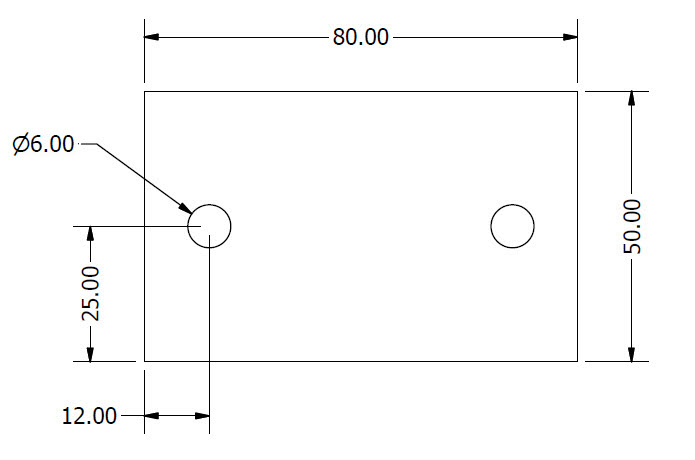
\includegraphics[width=0.5\textwidth]{2x6}
	\caption{Fyrsta reiknað tilvik}
	\label{fig::2x6}
\end{figure}

\subsubsection{Annað tilvik}

Vegna þess að fyrsta tilvik gékk ekki útaf leguspennum var athuga hvort 8 mm gat í stað 6 mm myndi standast forsendur okkar, sjá mynd \ref{fig::2x8}. Vegna því að aðeins ein breyting var gerð reiknast annað tilvikið líkt og það fyrsta.

\begin{itemize}
	\item Beygjaspenna á yfirborði við göt
	
	\[
	F = \frac{4 \sigma I}{l h} = {4 \cdot 210 MPa \cdot  \left({1 \over 12} \cdot 5 mm \cdot \left(50mm\right)^3 - {1 \over 12} 5 mm \cdot \left(8mm\right)^3\right) \over (160 mm + 12 mm) \cdot 50 mm} = \underline{5066N}
	\] 
	
	\item Skerspenna í bolta
	
	Á sama hátt og í fyrsta tilviki fæst sá kraftur sem veldur því að skerspennan í boltanum fari uppí flotspennu
	
	\[
	\sigma = {F_1^{''} \over A_b} \Rightarrow F = {4 S_{sy} A_b r_n \over l} = {4 \cdot {660MPa \over \sqrt{3}} \cdot {\pi \left(8mm\right)^2 \over 4} \cdot 28 mm \over 200 mm} = \underline{10726N}
	\]
	
	\item Leguspenna í efni
	
	Sá kraftur sem virkar á leguna er skerkrafturinn sem verkar á boltar, því verður leguspennan
	
	\[
	\sigma = {F_1^{''} \over bd} \Rightarrow F = {4 \sigma_{y} b d r_n \over l} = {4 \cdot 210 MPa \cdot 5 mm \cdot 8 mm \cdot 28 mm \over 200mm} = \underline{4704N}
	\]

\begin{figure}
	\centering
	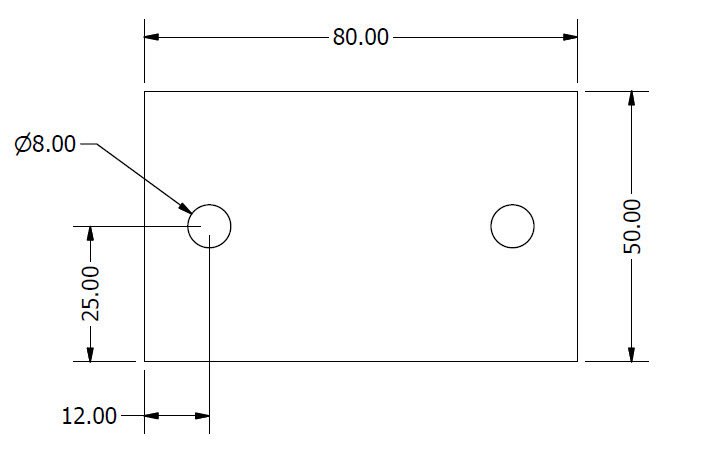
\includegraphics[width=0.5\textwidth]{2x8}
	\caption{Annað reiknað tilvik}
	\label{fig::2x8}
\end{figure}

\end{itemize}

Eftir þessa breytingu fara leguspennur ekki í flot við kraft lægri en $F_{y,p}$ og því eru forsendurnar uppfylltar. Aftur á móti munar ekki miklu á kraftinum sem veldur floti í legum og $F_{y,p}$. Því er þriðja hönnunin gerð.

\subsubsection{Þriðja tilvik}

Aðeins flóknari hönnun er gerð í þriðja skiptið. Þá eru fjórir boltar notaðir í stað tveggja, sjá mynd \ref{fig::4x6}. Vegna samhverfu dugir að reikna aðeins fyrir aðra hlið stykkisins og aðeins einn bolta þegar kemur að skerspennum og leguspennum. \fxnote{laga þetta orðalag!}

\begin{itemize}
	\item Beygjaspenna á yfirborði við göt
	
	Sá kraftur sem veldur floti fæst með jöfnu \ref{eq::1}. Eina breyting frá fyrri tilvikum er flatartregðuvægið, í þetta skiptið þarf að nota reglu Steiner's. Út frá því fæst að flatartregðuvægið er $I = {1 \over 12}bh^3 - 2\left({1 \over 12}bd^3)\right)$. Flatartregðuvægið er því
	
	\[
	F = \frac{4 \sigma I}{l h} = {4 \cdot 210 MPa \cdot \left({1 \over 12} \cdot 5 mm \cdot \left(50mm\right)^3 - 2 \cdot \left({1 \over 12} \cdot 5 mm \cdot \left(6mm\right)^3\right)\right) \over (160 mm + 12 mm) \cdot 50 mm} = \underline{5070N}
	\] 
	
	\item Skerspenna í bolta
	
	Vegna samhverfu bitans fæst sami kraftur í alla bolta. \fxnote{Bæta við orðum hér! Vissi ekki alveg hvað ég átti að segja}
	
	\[
	F_1^{''} = F_2^{''} = F_3^{''} = F_4^{''} = {Mr_n \over 4r_n^2} = {{F \over 2}l \over 4 r_n} 
	\]
	
	Í þessu tilviki er $r_n = \sqrt{(40mm - 12mm)^2 + (25mm - 13mm)^2} = 30.5 mm$. Því fæst sá kraftur sem veldur floti í boltum sé 
		\[
		\sigma = {F_1^{''} \over A_b} \Rightarrow F = {8 S_{sy} A_b r_n \over l} = {8 \cdot {660MPa \over \sqrt{3}} \cdot {\pi \left(6mm\right)^2 \over 4} \cdot 30.5 mm \over 200 mm} = \underline{13144N}
		\]
	
	
	\item Leguspenna í efni
\end{itemize}

\begin{figure}
	\centering
	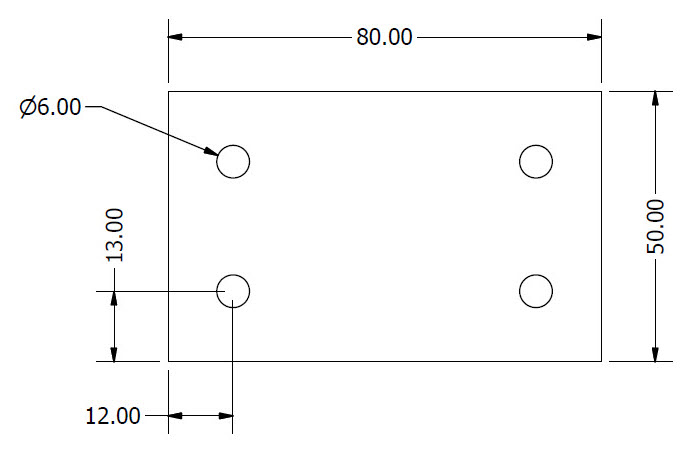
\includegraphics[width=0.5\textwidth]{4x6}
	\caption{Þriðja reiknað tilvik}
	\label{fig::4x6}
\end{figure}